\svnid{$Id$}
\chapter{Nitrite Reduction in \Nm{}}
\label{chap:nitritereduction}

%In the case of this dataset, nitrite reduction has been modelled very well, but nitric oxide (and to a small extent, oxygen) has not been [Caveat, this may change when the cluster does eventually spit out the complete trajectory. This then could be moved into the discussion about why priors are important]. Not shown in Figure \ref{fig:no2sim} is the concentration of nitric oxide as nitrite is reduced. Unfortunately the parameter set used to generate the solved output assigned a very low value to the concentration of NorB (even though this should have been being expressed), thus the nitric oxide produced by reduction of nitrite does not itself get reduced, and towards the end of the dataset would be lethal to the culture. In this case, a different prior distribution should have been used for NorB concentration, as it was known beforehand that NorB concentration would be non-zero. This is an example of why the prior distributions are important.

\section{Microerobic Nitrite Reduction}
% \subsection{Introduction}
% \subsection{Results}
% \subsection{Discussion}
% \section{\texorpdfstring{Microaerobic Nitrite Reduction in \textit{norB$^\textrm{-}$} mutant}{Microaerobic Nitrite Reduction in norB- mutant}}
% \subsection{Introduction}
% \subsection{Results}
% \subsection{Discussion}
% \section{\texorpdfstring{Aerobic Nitrite Reduction in \textit{nsrR$^\textrm{-}$} mutant}{Aerobic Nitrite Reduction in nsrR- mutant}}
\subsection{Introduction}

The last datasets to be used in the iterative approach to parameter estimation was of cultures able to respire nitrite in addition to oxygen. In these cultures nitrite was added to a culture already respiring oxygen to observe both the rate of nitrite reduction, and the effect on oxygen respiration caused by the production of nitric oxide. These datasets were the most complex in terms of the information contained within them and the number of model components needed to solve them. In addition to the components being used to model nitric oxide reduction, the nitrite reduction pathway is also active. The portions of the ETC relating to nitrite reduction are shown graphically in Figure \ref{fig:no2_resp_chain}. However since \Nsm{} is incapable of respiring anaerobically, in actual fact the entire pathway is required, using oxygen nitric oxide and nitrite reduction.
\begin{figure}[tbp]
  \centering
    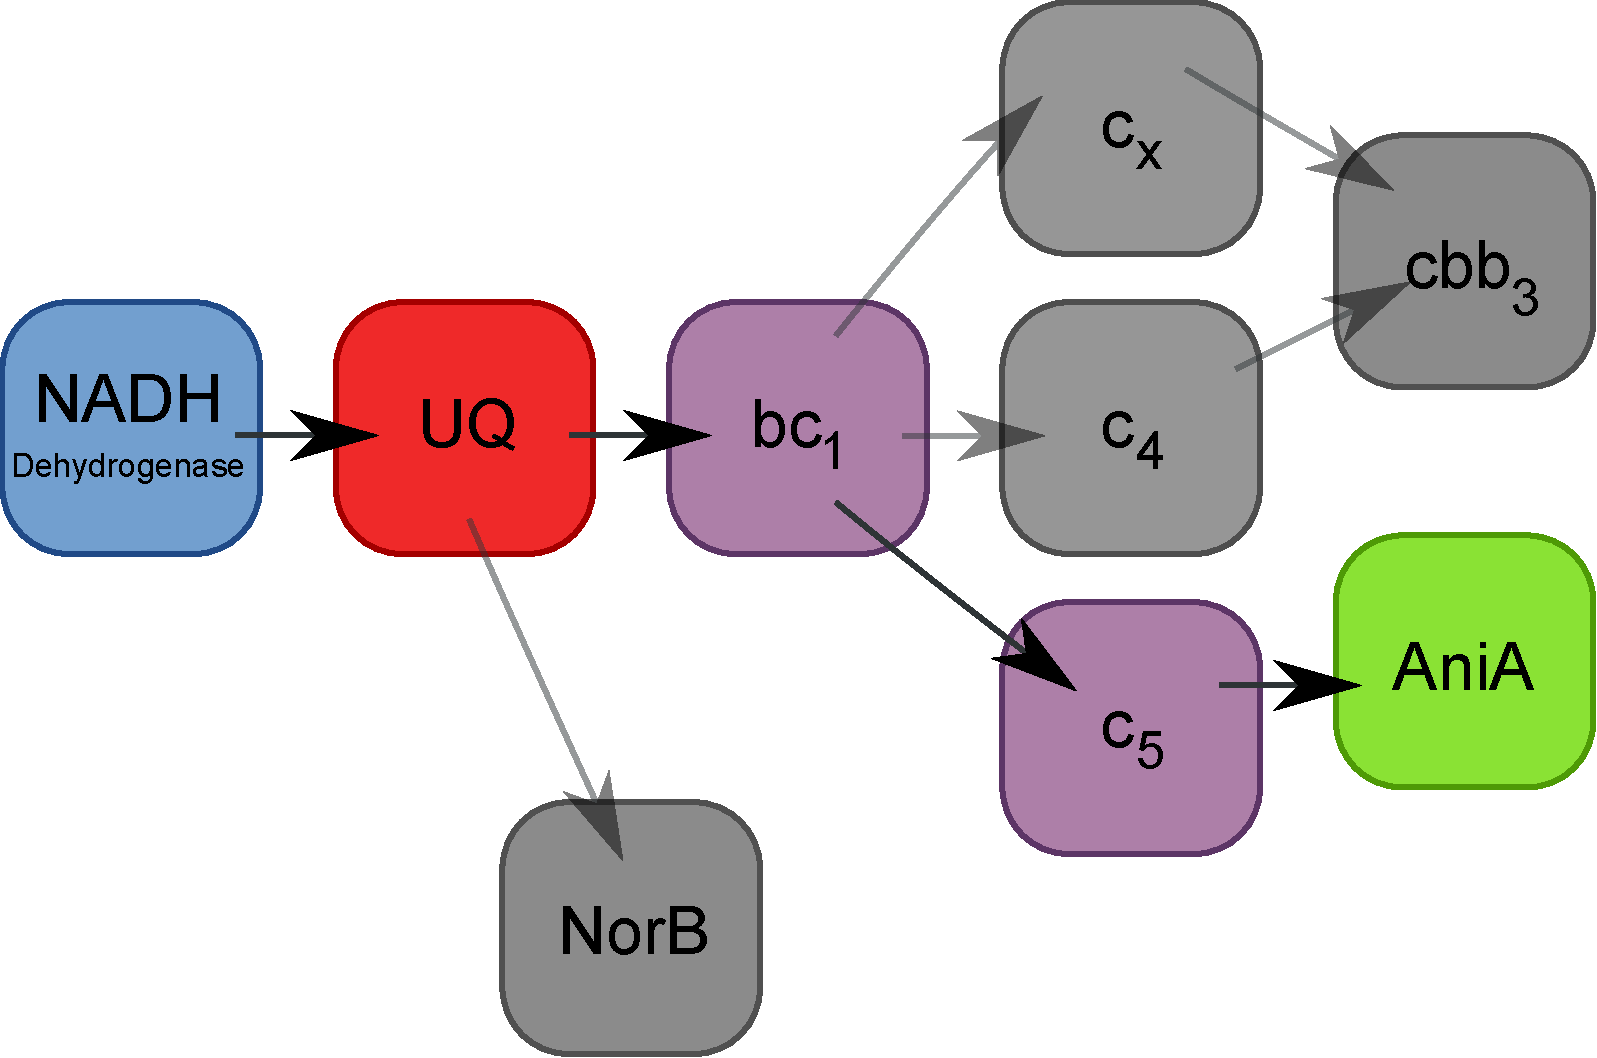
\includegraphics[width=14cm]{07-nitritereduction/data/no2_resp_chain.pdf}
    \caption[Nitrite reducing electron transport chain of \Nm{}]{{\bf Nitrite reducing electron transport chain of \Nm{}.} This shows the complete electron transport chain of \Nsm{} with the components irrelevant to nitrite reduction greyed out. In the mathematical model all of the purple elements (cytochromes) are amalgamated into one entity.
  \label{fig:no2_resp_chain}}
\end{figure}

\noindent The equations that describe this portion of the ETC are:
\begin{eqnarray*}
\frac{d[O_2]}{dt} & = & \beta(1-[O_2]/K_O) - k_{1}[C_a][O_2]\\
\frac{d[Q_a]}{dt} & = & g([Q] - [Q_a]) - l_3[Q_a]([B] - [B_a]) - f[Q_a]([X]-[X_a])\\
\frac{d[X_a]}{dt} & = & -k_3([C] - [C_a] - [C_X])[X_a]  - m_3([A] - [A_a])[X_a] + f[Q_a]([X]-[X_a])\\
\frac{d[C_a]}{dt} & = & k_3([C] - [C_a] - [C_X])[X_a] - k_{1}[C_a][O_2] - k_5[C_a][NO] + k_6[C_X]\\
\frac{d[NO]}{dt} & = & m_{1}[NO_2^-][A_a] - l_1[NO][B_a] - k_5[C_a][NO] + k_6 [C_X] - \gamma[NO]\\
\frac{d[NO_2^-]}{dt} & = & - m_{1}[NO_2^-][A_a]\\
\frac{d[C_X]}{dt} & = & k_5[C_a][NO] - k_6 [C_X]\\
\frac{d[A_a]}{dt} & = & m_3([A] - [A_a])[X_a]- m_{1}[NO_2^-][A_a]\\
\frac{d[B_a]}{dt} & = & l_3[Q_a]([B] - [B_a]) - l_1[NO][B_a]
\end{eqnarray*}

These equations describe the change in concentration of nitrite over time, which is the experimentally observed value (in addition to the afore modelled oxygen and nitric oxide). Also modelled is the reduction state of AniA. This represents the complete mathematical model not including any transcriptional parameters.

\subsection{Experimental Results}
Generating datasets for Nitrite reduction could be performed in with two different cultures; an aerobic NsrR deficient mutant, or microaerobic wild-type. Microaerobic cultures appeared to grow very poorly during the course of this work and in most cases did not survive the transition from being in the incubator to being moved to the electrode chamber. Therefore an $nsrR^-$ mutant was used instead of the wild-type. This mutant expresses AniA and NorB in a constitutive manner, removing the necessity for growing the cultures in microaerobic conditions. The cultures were grown in aerobic conditions until mid-log phase growth had been achieved. This corresponded to an $OD_{600}$ of $0.3-0.9$ and usually required an incubation period of roughly 3 hours. Once the required cell density had been obtained the culture was transferred to the electrode chamber, Sodium Nitrite was added to a concentration of 1 mM and the nitrite and oxygen concentrations recorded as the culture respired. Unfortunately nitric oxide concentrations could not be recorded as the NO electrode had failed and could not be replaced.

In addition to the datasets obtained from $nsrR^-$ mutant cultures, a further dataset was obtained from \citet{Rock2005} which showed oxygen and nitric oxide concentrations in a microaerobic wild-type culture where nitrite is added partway through aerobic respiration. The datasets generated and used for parametrisation of this portion of the model are shown in Figures \ref{fig:nitriteds1} \& \ref{fig:nitriteds2}.

The dataset in Figure \ref{fig:nitriteds1} shows an $nsrR^-$ mutant which has had 1mM nitrite added at $t=0s$. Nitrite reduction proceeds linearly and at quite a high rate. Oxygen starts linearly but then slows down presumably as nitric oxide is produced ans inhibits \cbbthree{}. It is also possible that given the high rate of nitrite reduction large quantities of nitric oxide are being produced which will react directly with oxygen as described in Chapter \ref{chap:noreduction} affecting the rate of observed oxygen reduction.

The dataset in Figure \ref{fig:nitriteds2} shows a wild-type culture grown in denitrifying conditions, so that it is expressing both AniA and NorB. Nitrite is added at time $t\approx200s$ to a concentration of $\approx 1$ mM (Moir, private communication). Upon nitrite addition a small decrease in oxygen respiration rate is observed, and a large increase in nitric oxide occurs as nitrite is reduced. Nitric oxide is then maintained at a fairly constant level until oxygen is fully reduced at which point a further increase in nitric oxide concentration is observed. It is posited that this final increase in NO concentration is because the electrons that were being pulled through the oxygen respiration pathway are now free to be drawn to AniA allowing more nitrite reduction to take place.

\begin{figure}[tbp]
 \centering
 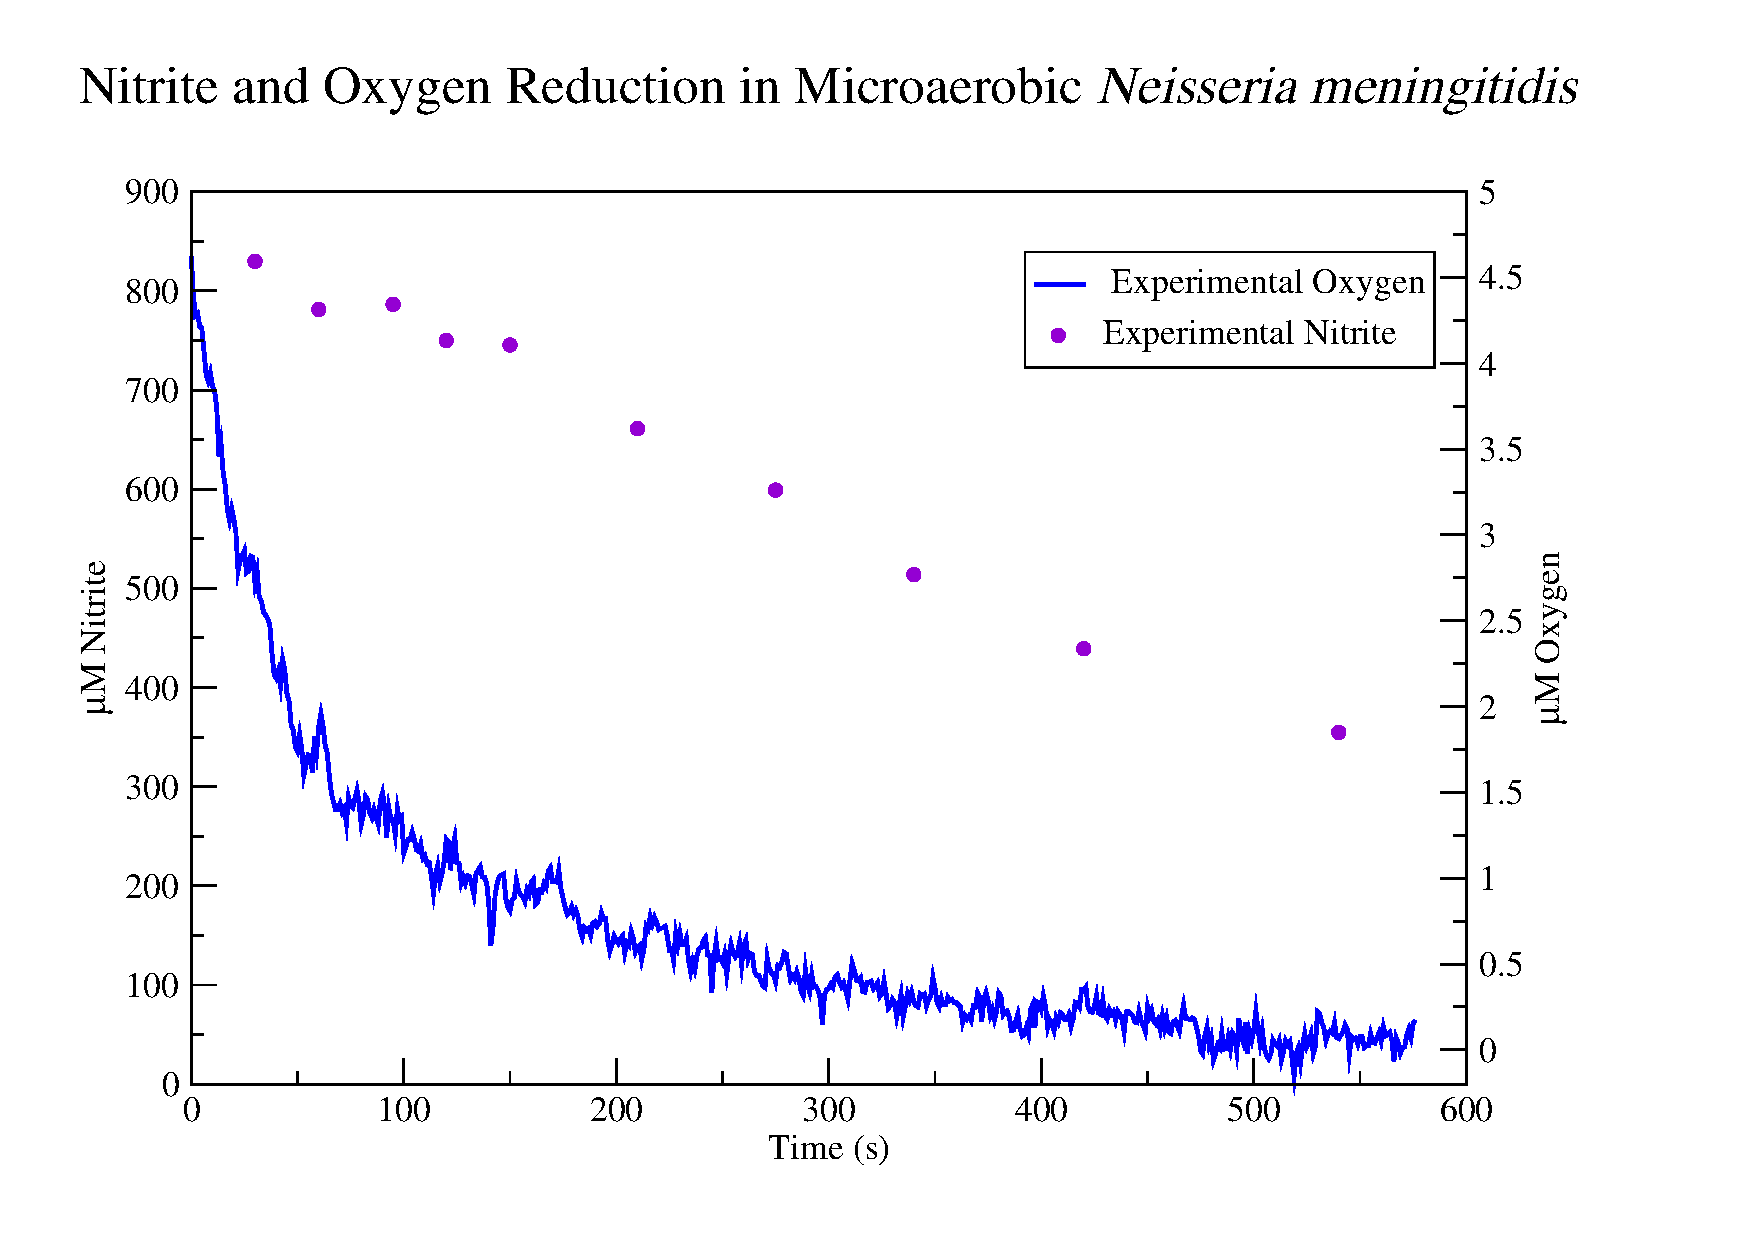
\includegraphics[height=10cm]{./07-nitritereduction/data/dataset1.pdf}
 % dataset1.pdf: 842x595 pixel, 72dpi, 29.70x20.99 cm, bb=0 0 842 595
 \caption[Nitrite Reduction in \Nsm{}]{{\bf Nitrite Reduction in \Nsm{}.} This dataset shows the effect on oxygen respiration of nitrite respiration as nitric oxide is produced. This culture is an $nsrR^-$ mutant which is expressing AniA and NorB in an essentially constitutive manner.
 \label{fig:nitriteds1}}
\end{figure}

\begin{figure}[tbp]
 \centering
 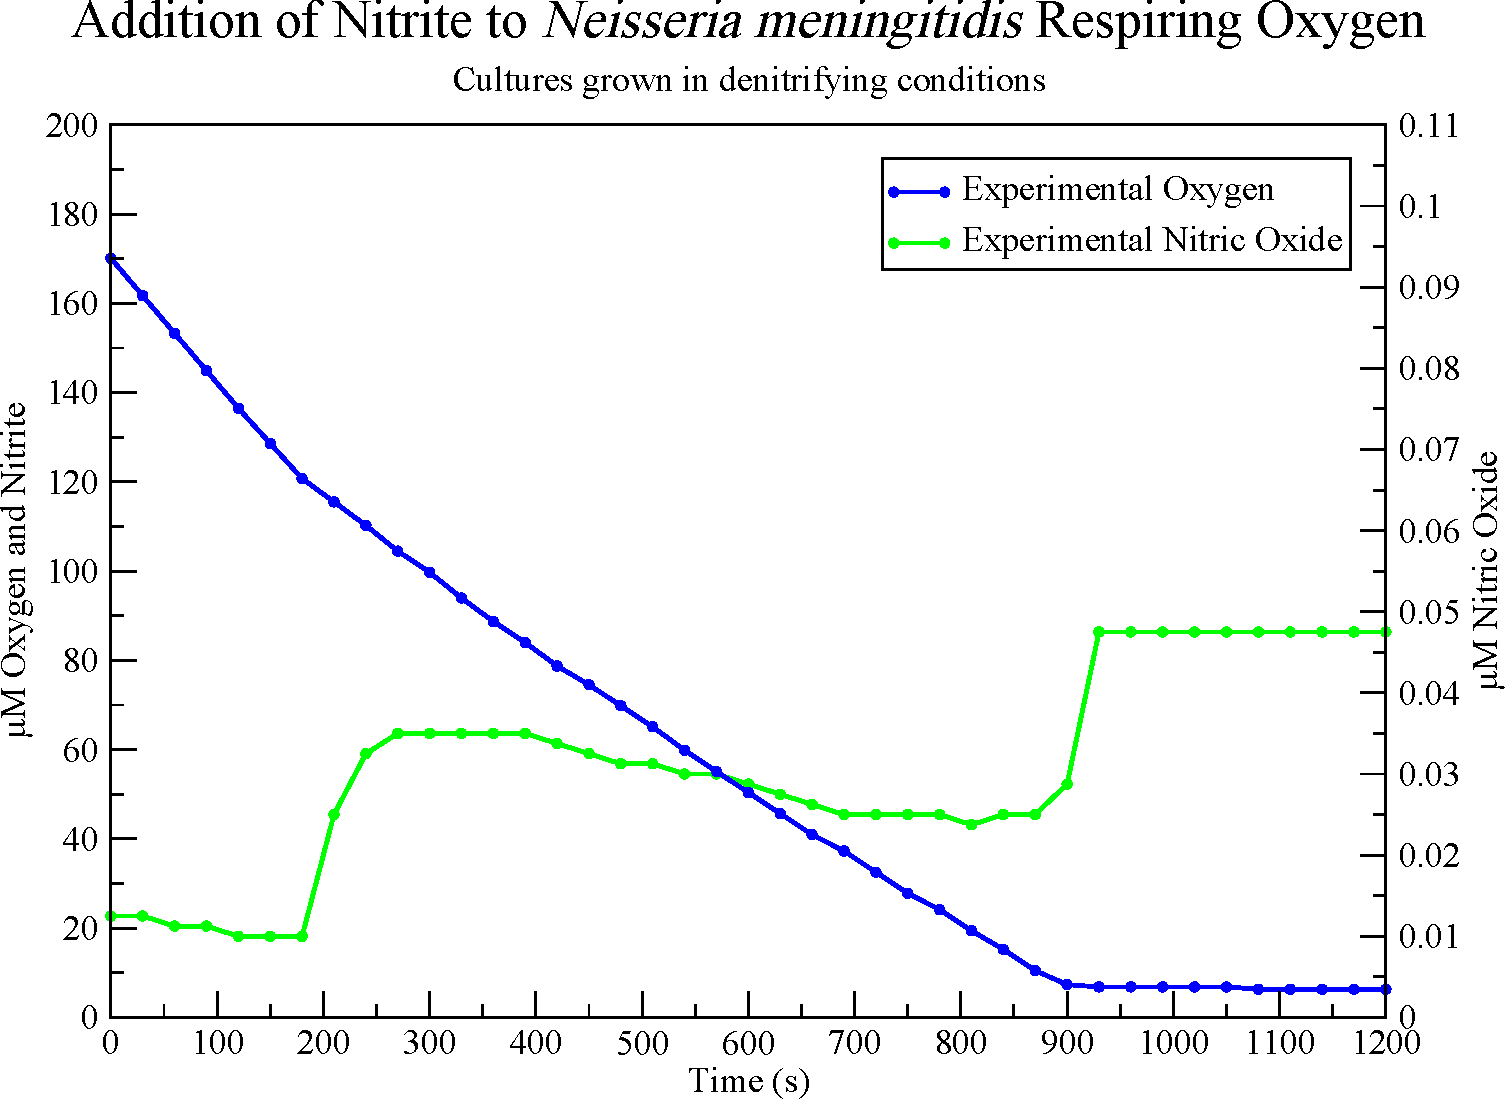
\includegraphics[height=10cm]{./07-nitritereduction/data/dataset2.pdf}
 % dataset1.pdf: 842x595 pixel, 72dpi, 29.70x20.99 cm, bb=0 0 842 595
 \caption[Nitrite Reduction in \Nsm{}]{{\bf Nitrite Reduction in \Nsm{}.} This dataset shows the effect of nitrite addition to an aerobically respiring culture. Nitrite is added at 200s. Oxygen and Nitric Oxide data-points are recorded with much less frequency than in previous datasets hence the inclusion of dots on the plot.
 \label{fig:nitriteds2}}
\end{figure}

\subsection{Prior Probability Distributions}

As described previously all parameters much have an associated prior probability distribution. The posterior probability distributions from Chapter \ref{chap:noreduction} were used as prior probability distributions in theis chapter. Where new parameters were introduced, the distributions were generated based on published literature values which are noted in Chapter \ref{chap:model}. When using literature values the prior probability distributions were generated according to the same scheme as in Chapter \ref{chap:oxygenreduction}. The values required to create idealised lognormal probability distributions for each parameters are shown in Table \ref{tab:nitrite_prior_table}.

\begin{table}[ht]%needs to be 'here' as section is short
\renewcommand{\arraystretch}{1.5}
\begin{center}
\begin{tabular}{cccc|cccc}
\toprule
\textbf{Parameter} && ${\bar{x}}$ & $\sigma$ & \textbf{Parameter} && ${\bar{x}}$ & $\sigma$\\
\midrule
$k_1$ && 417.88 & 31.172 & g && 0.857 & 0.086\\
$k_3$ && 4.65 & 0.619 & f && 8.398 & 1.237\\
$l_1$ && 13.12 & 8.321 & $\gamma$ && 0.00014 & $4.67\times 10^{-6}$\\
$l_3$ && 0.058 & 0.021 & Q && 7.06 & 1.317\\
$m_1$ && 1 & 1 & X && 27.45 & 12.08\\
$m_3$ && 4.8 & 0.2 & A && 0.137 & 0.048\\
$k_5$ && 1741.8 & 1822.0 & B && 0.137 & 0.048\\
$k_6$ && 1.076 & 1.473 & C && 0.071 & 0.029\\
$\beta$ && 0.00014 & $4.67\times 10^{-6}$\\
\bottomrule
\end{tabular}
\end{center}
\caption[Prior Probability Table]{{\bf Prior Probability Table} This table shows the prior means and standard deviations used to create lognormal distributions to be used as the prior probability distributions.
\label{tab:nitrite_prior_table}}
\end{table}

The initial probability distributions used to start the Monte-Carlo runs are shown in Figure \ref{fig:nitrite_priors1}.

\begin{figure}[tbp]
 \centering
 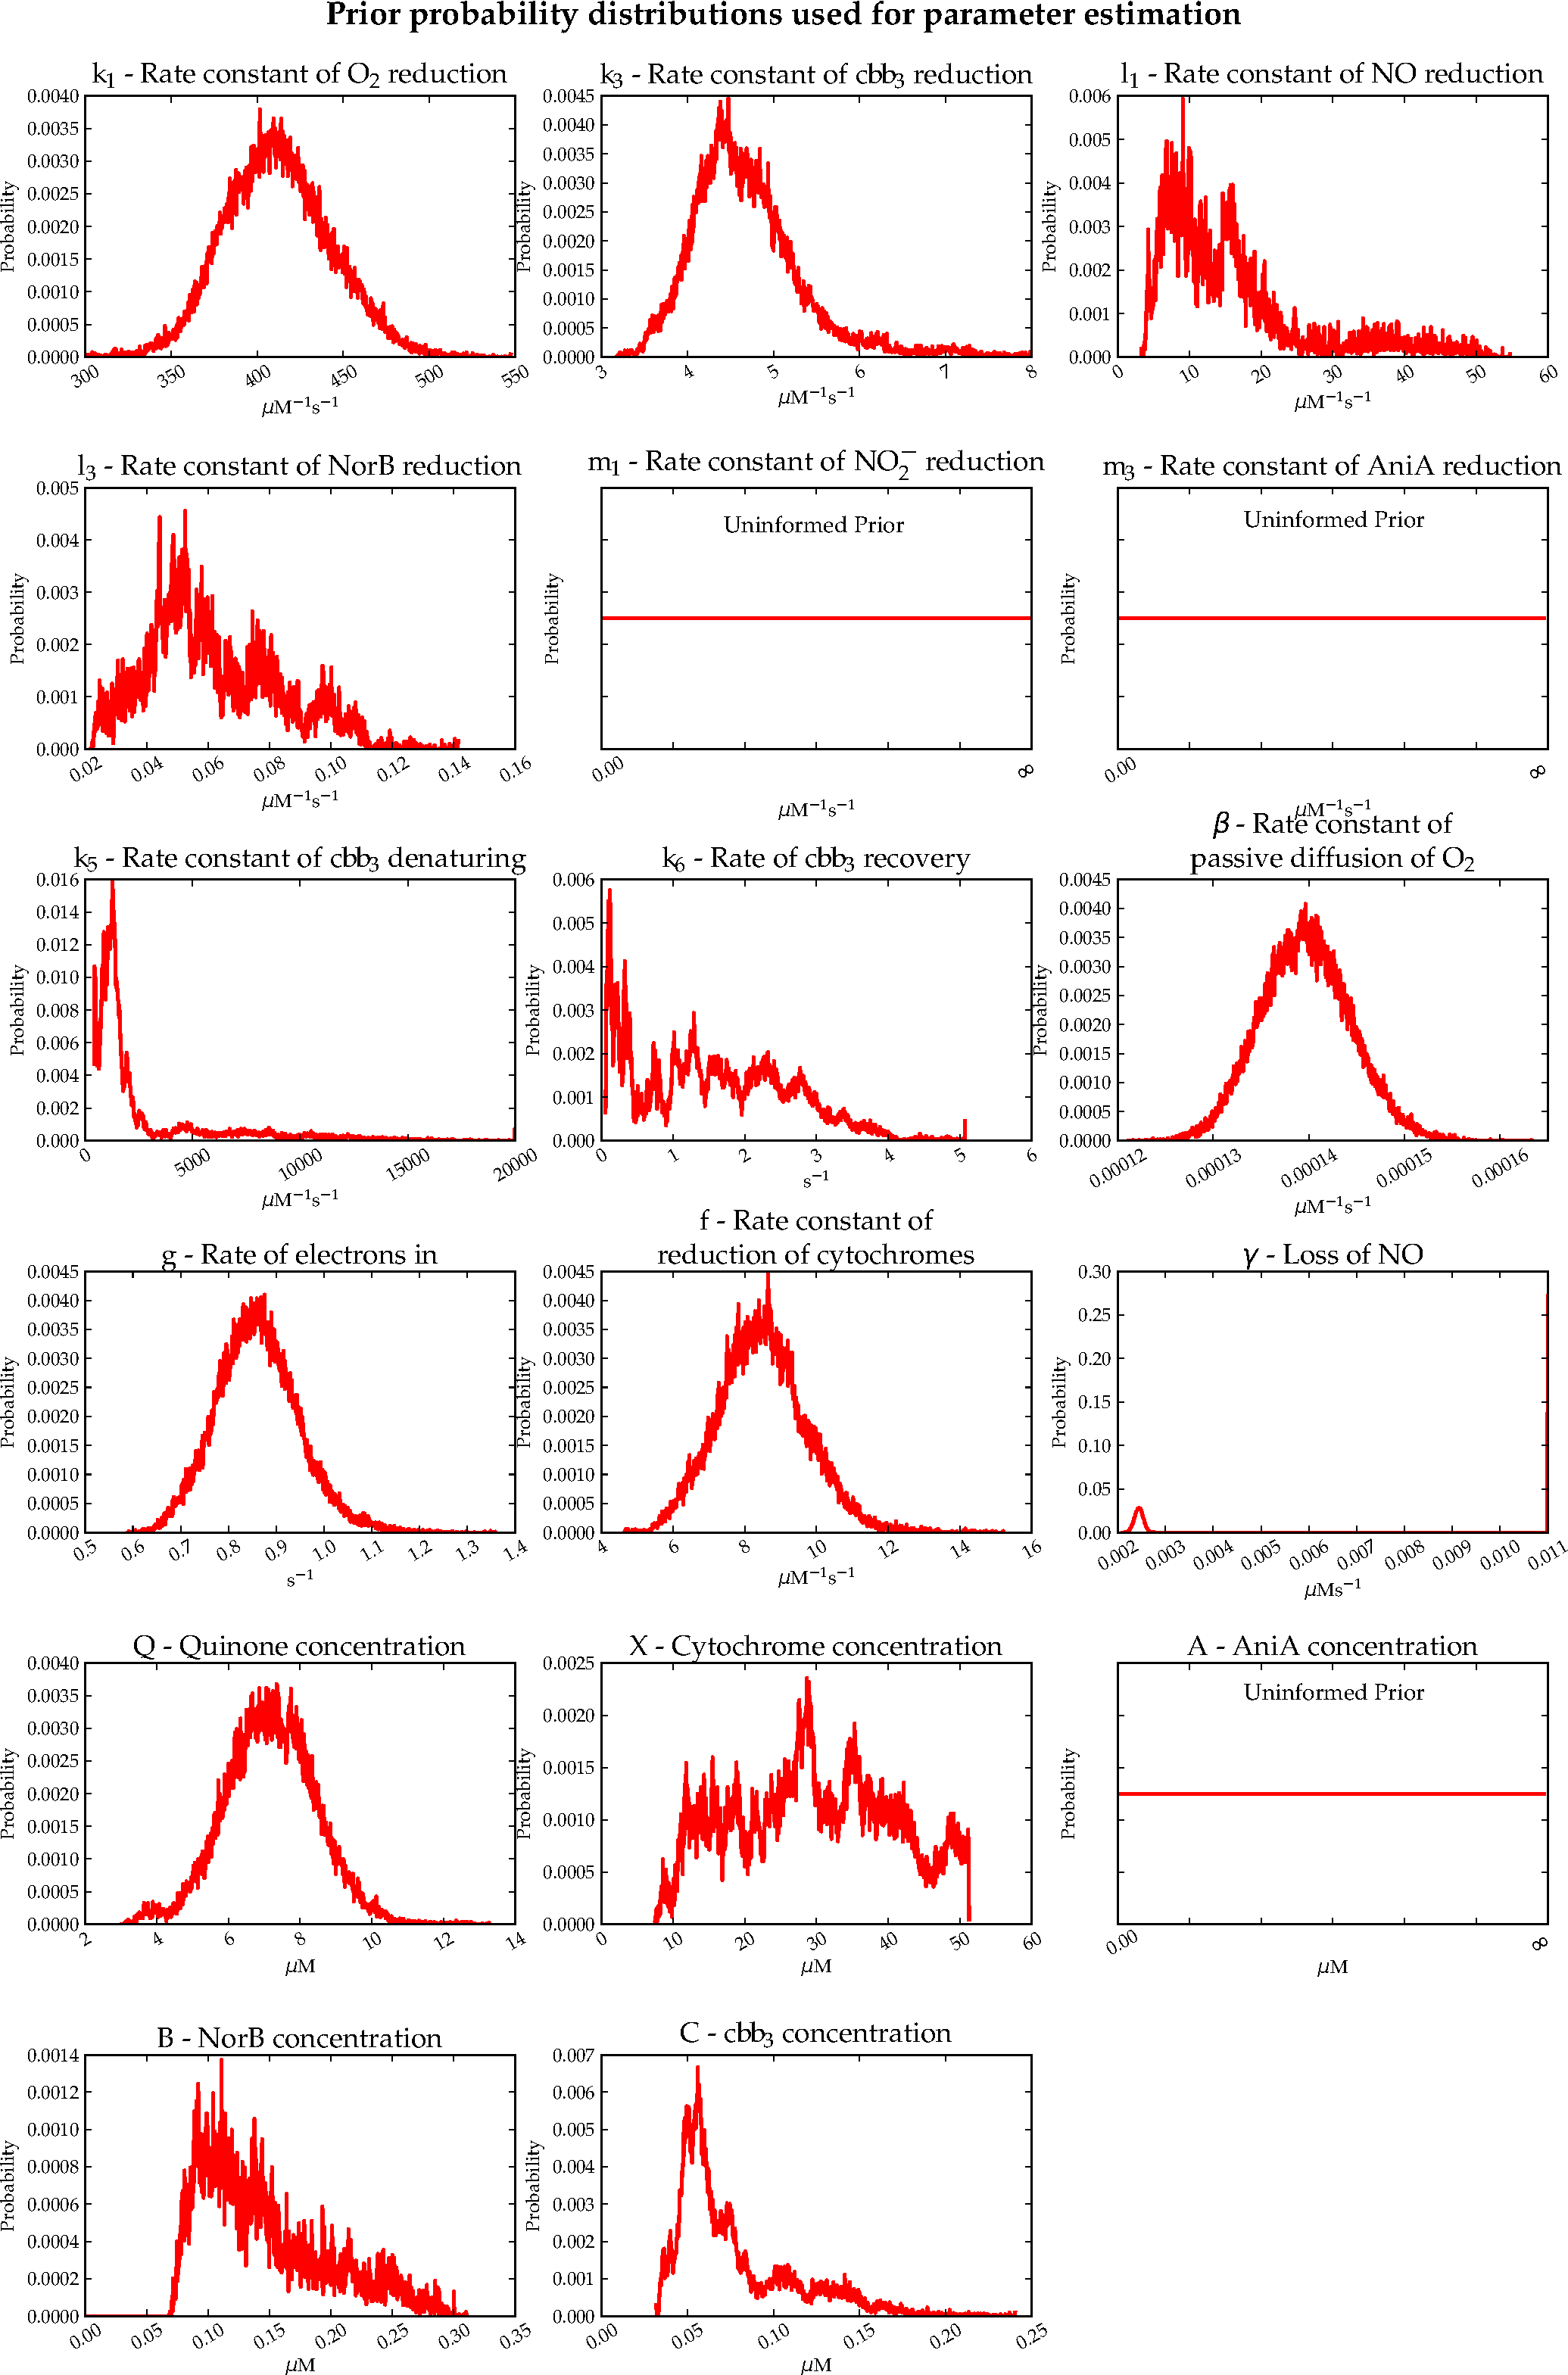
\includegraphics[width=15cm, trim=0cm 0cm 0cm 0cm]{./07-nitritereduction/data/priors1.pdf}
 % priors.pdf: 1008x1008 pixel, 72dpi, 35.56x35.56 cm, bb=0 0 1008 1008
 \caption[Prior probability distributions for microaerobic oxygen and nitrite reduction]{{\bf Prior probability distributions for microaerobic oxygen and nitrite reduction}. These are the probability distributions used as priors by the parameter estimation algorithm.
 \label{fig:nitrite_priors1}}
\end{figure}
\afterpage{\clearpage}

\subsection{Parameter Estimation Results}
The parameter estimation process was run in the same fashion as that described in Chapters \ref{chap:oxygenreduction} \& \ref{chap:noreduction}. The 2 experimental datasets were run 20 times (each) for 20,000 iterations using the prior probability distributions shown in Figure \ref{fig:nitrite_priors1}. The solved output from datasets 1 and 2 are shown in Figures \ref{fig:nitrite_ds1_solved1} and \ref{fig:nitrite_ds2_solved1} respectively. Given the apparent poor fitting of the solved outputs shown in both of these figures, plots of the redox states for both of these datasets are shown in Figures \ref{fig:nitrite_ds1_redox1} and \ref{fig:nitrite_ds2_redox1}.

\begin{figure}[tbp]
 \centering
 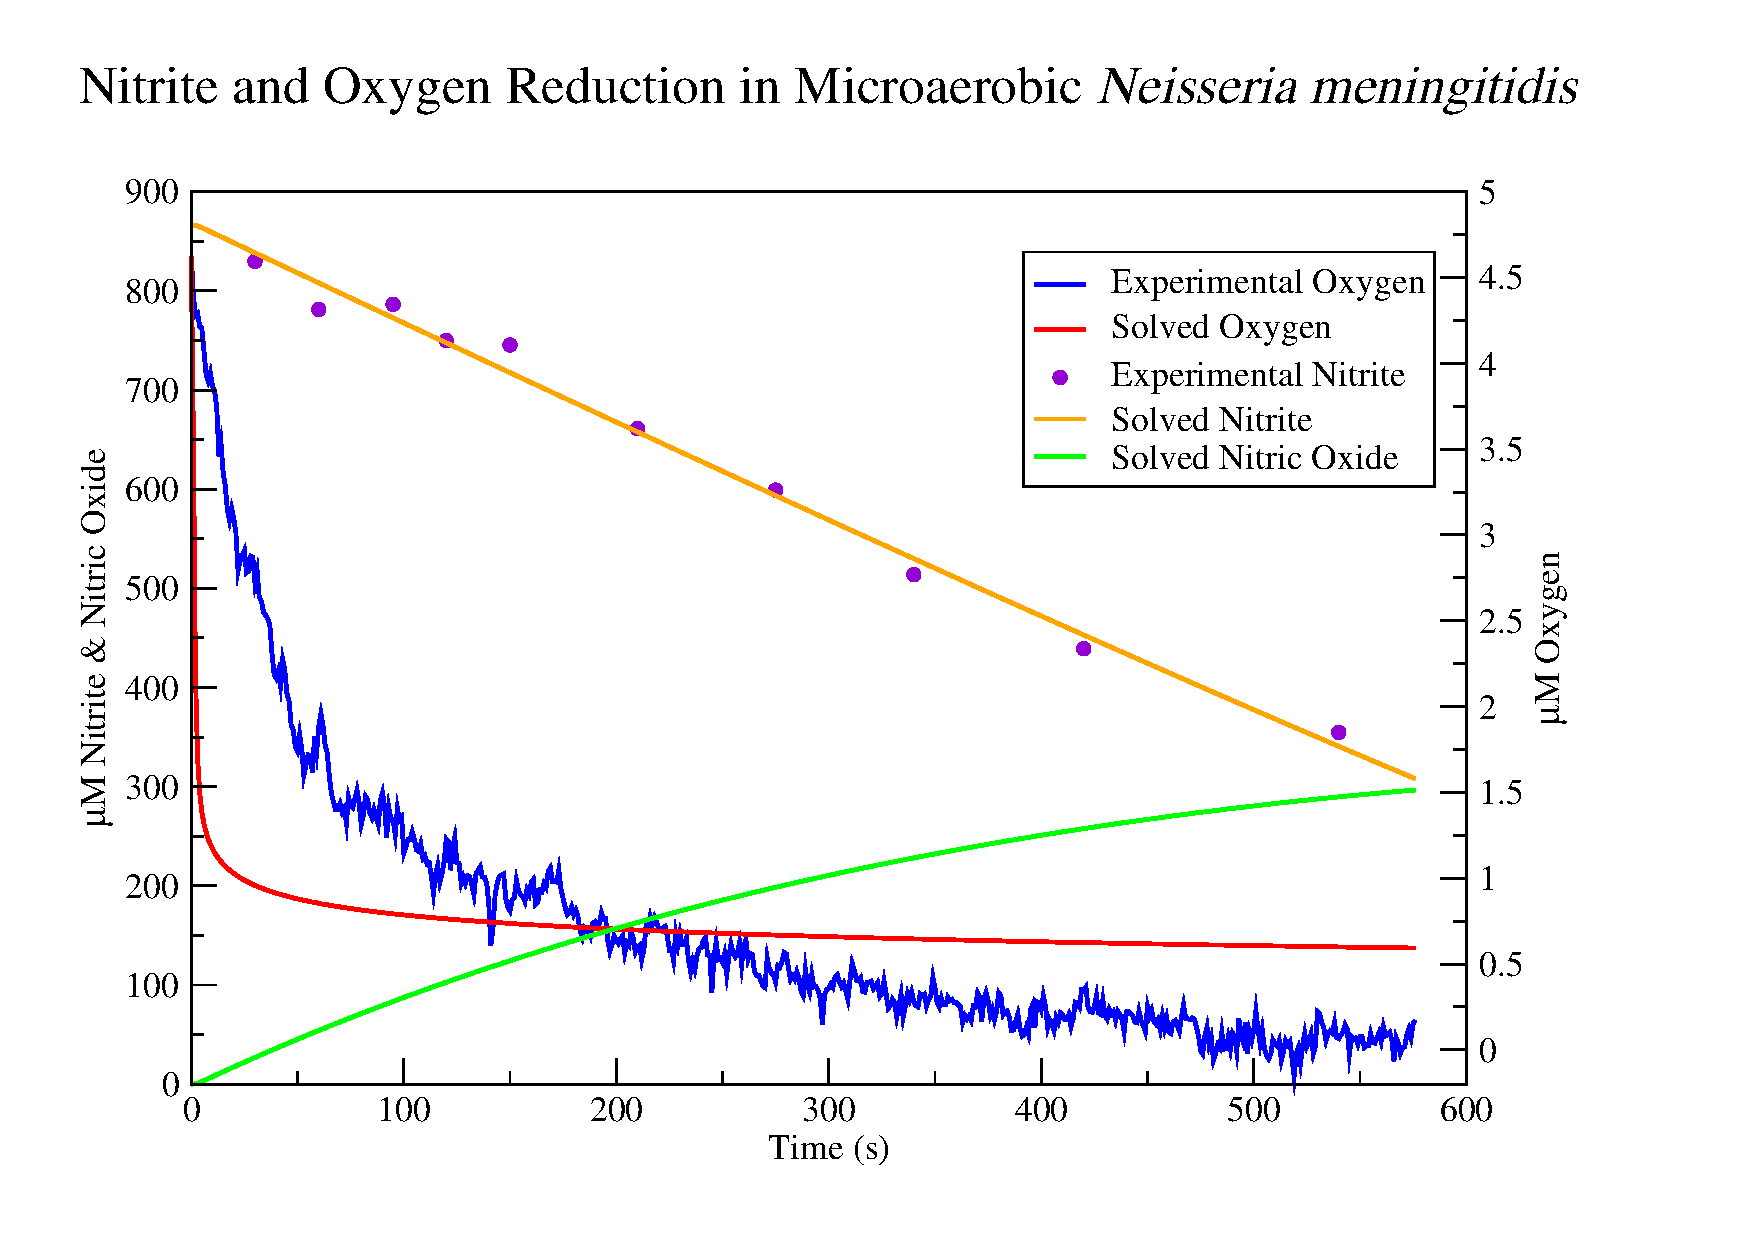
\includegraphics[height=10cm, trim=1cm 1cm 3cm 1cm, clip=true]{./07-nitritereduction/data/dataset1-1.pdf}
 % dataset1-1.pdf: 842x595 pixel, 72dpi, 29.70x20.99 cm, bb=0 0 842 595
 \caption[Solved Nitrite Reduction in \Nsm{}]{{\bf Solved Nitrite Reduction in \Nsm{}}. This figure shows the first attempt at fitting the model to experimental data. Nitrite reduction is being modelled well, whereas oxygen reduction is being modelled quite poorly as the solved data shows to high a rate of oxygen reduction. Nitric oxide is solved purely as a product of nitrite reduction and is not compared to any experimental data.
  \label{fig:nitrite_ds1_solved1}}
\end{figure}

The solved data shown in Figure \ref{fig:nitrite_ds1_solved1} doesn't fit particularly well to the experimental data. Nitrite reduction appears to be modelled well as it is a simple linear reduction. Oxygen reduction however is modelled very poorly. The initial rate of oxygen reduction is too high, and the reduction in rate is too fast. The halting of oxygen reduction is due to the amount of nitric oxide being produced by the reduction of nitrite. This level of nitric oxide quickly inhibits the \cbbthree{} totally as can be seen by the large level of nitric oxide concentration in Figure \ref{fig:nitrite_ds1_solved1} and in the redox plot in Figure \ref{fig:nitrite_ds1_redox1}. The redox plots show that essentially all the electrons in the system are flowing to the nitrite reduction pathway. Nitric oxide is progressing as fast as possible based on the electron flow into NorB. NorB stays in a permanently oxidised states suggesting that the reduction activity of NorB is faster than the rate of reduction of NorB itself. The level of NorB is also not easily modelled correctly using this data as no information is available about the actual levels of nitric oxide being produced during nitrite reduction.

\begin{figure}[tbp]
 \centering
 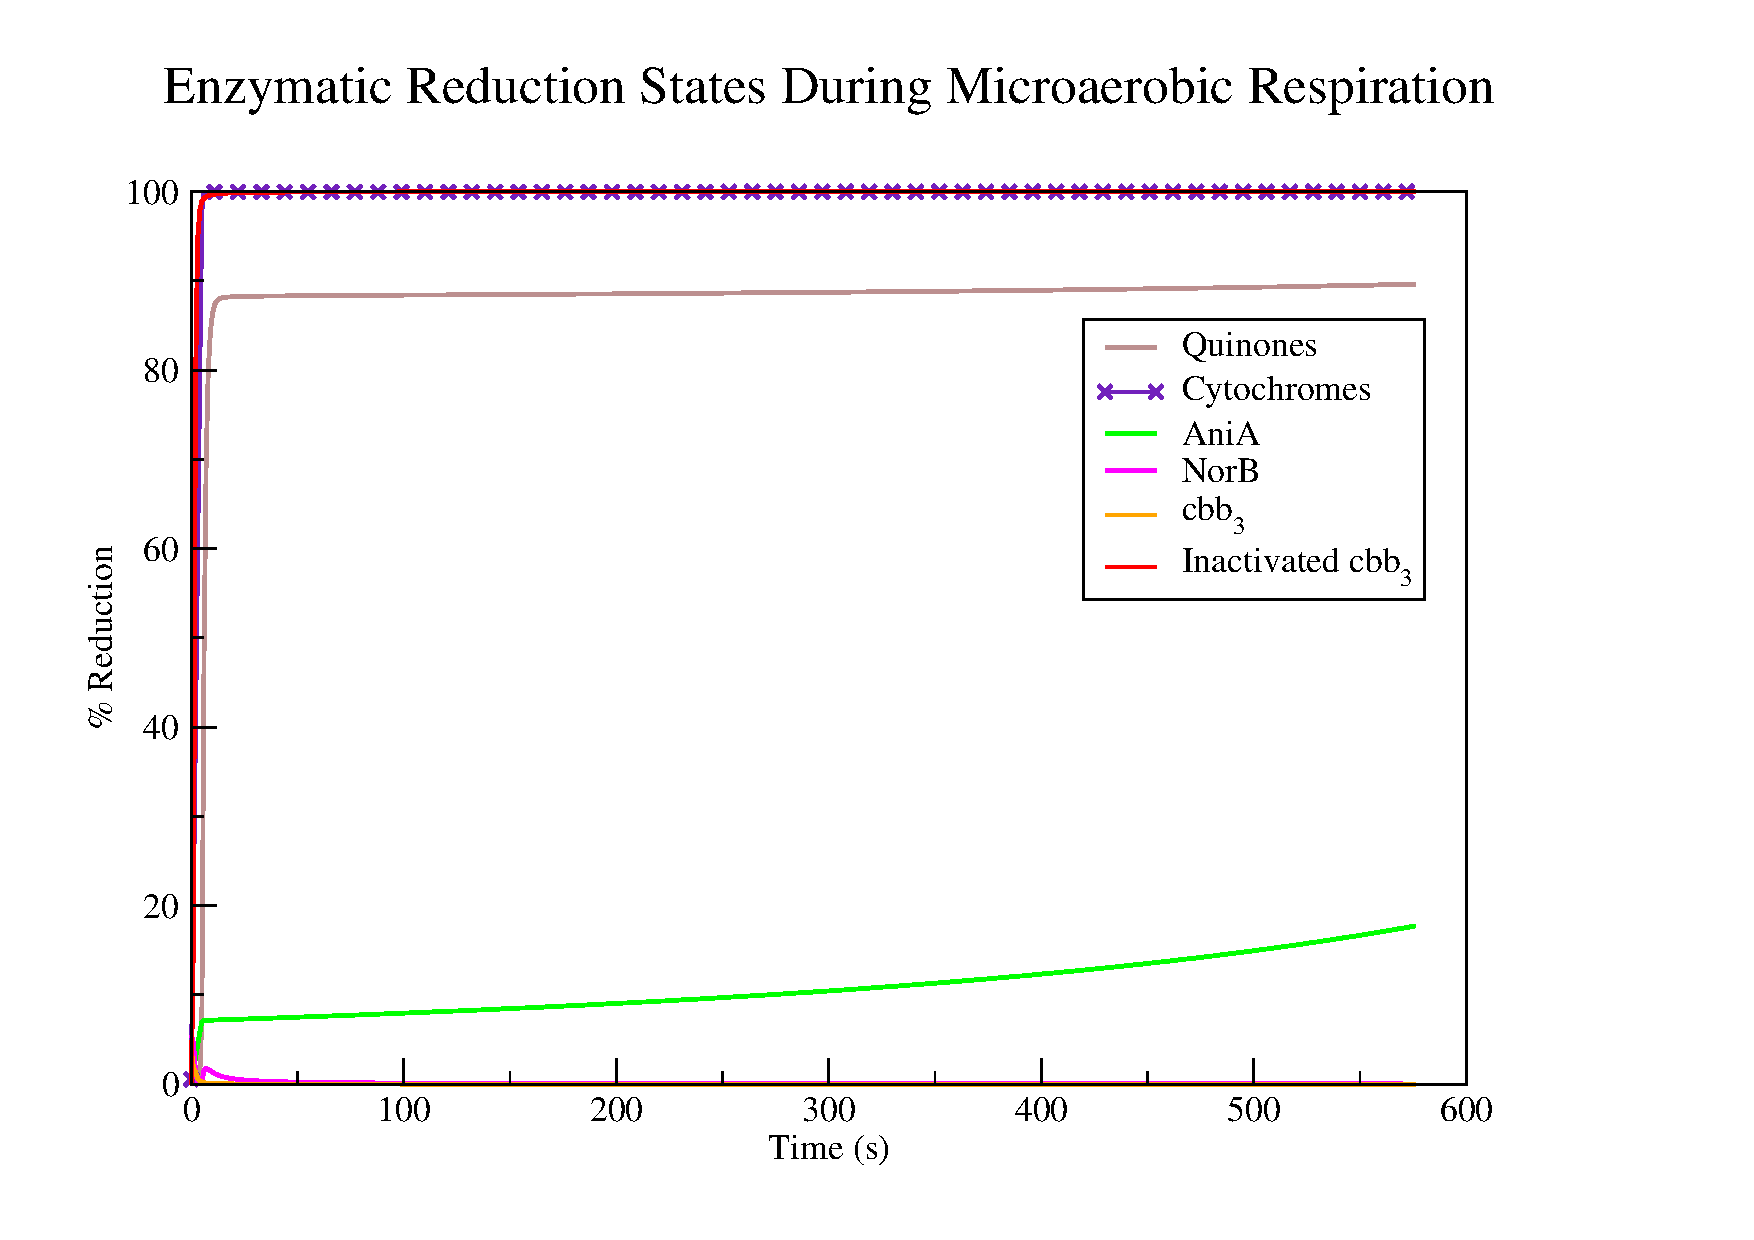
\includegraphics[height=10cm, trim=1cm 1cm 3cm 1cm, clip=true]{./07-nitritereduction/data/dataset1redox-1.pdf}
 % dataset1redox-1.pdf: 842x595 pixel, 72dpi, 29.70x20.99 cm, bb=0 0 842 595
 \caption[Reduction States During Nitrite Reduction]{{\bf Reduction States During Nitrite Reduction}. This figure shows how the reduction states of the enzymes involved in nitrite reduction change during respiration.
  \label{fig:nitrite_ds1_redox1}}
\end{figure}

The solved data in Figure \ref{fig:nitrite_ds2_redox1} appears to fit oxygen reduction quite well but fails to fit nitric oxide reduction almost entirely. The most significant feature, that nitric oxide should increase when oxygen reduction ceases is missing. The redox state plot in Figure \ref{fig:nitrite_ds2_redox1} suggests the reason for the lack of this feature. The cytochromes appear to be in a completely reduced state shortly after the start of the simulation. This permanently reduced state means that when oxygen reduction ceases there is essentially no difference to the flow of electrons to either NorB or AniA. This suggests that parameters $g$ and $f$, the reduction of cytochromes and the reduction of the quinone pool are too high, leading to the permanent reduction of both those components. The nitrite levels are equally difficult to model as nitric oxide in the previous dataset as the levels are unknown.

\begin{figure}[tbp]
 \centering
 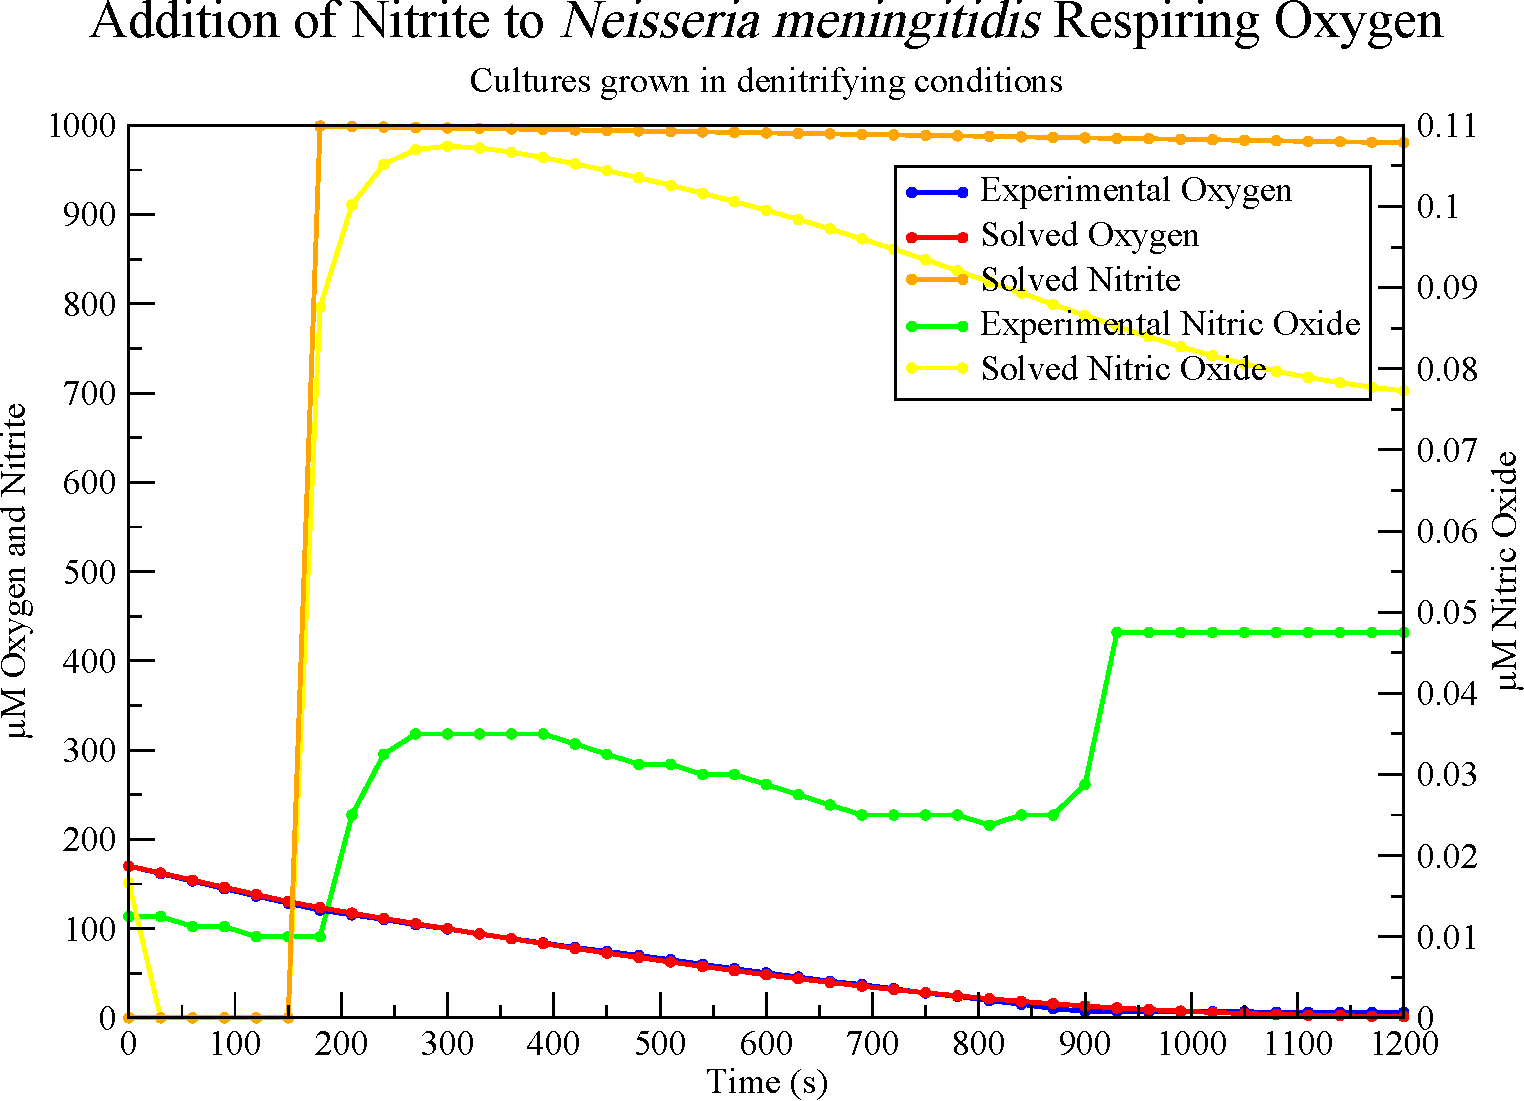
\includegraphics[height=10cm, trim=1cm 1cm 3cm 1cm, clip=true]{./07-nitritereduction/data/dataset2-1.pdf}
 % dataset2-1.pdf: 842x595 pixel, 72dpi, 29.70x20.99 cm, bb=0 0 842 595
 \caption[Effect of Nitrite Addition on Aerobically Respiring Cultures]{{\bf Effect of Nitrite Addition on Aerobically Respiring Cultures}. This figure shows the first attempt at fitting the model to experimental data. Oxygen respiration appears appears to be modelled quite well, but nitric oxide is being modelled particularly badly. The most significant feature of the nitric oxide dataset is absent in the solved data.
  \label{fig:nitrite_ds2_solved1}}
\end{figure}

\begin{figure}[tbp]
 \centering
 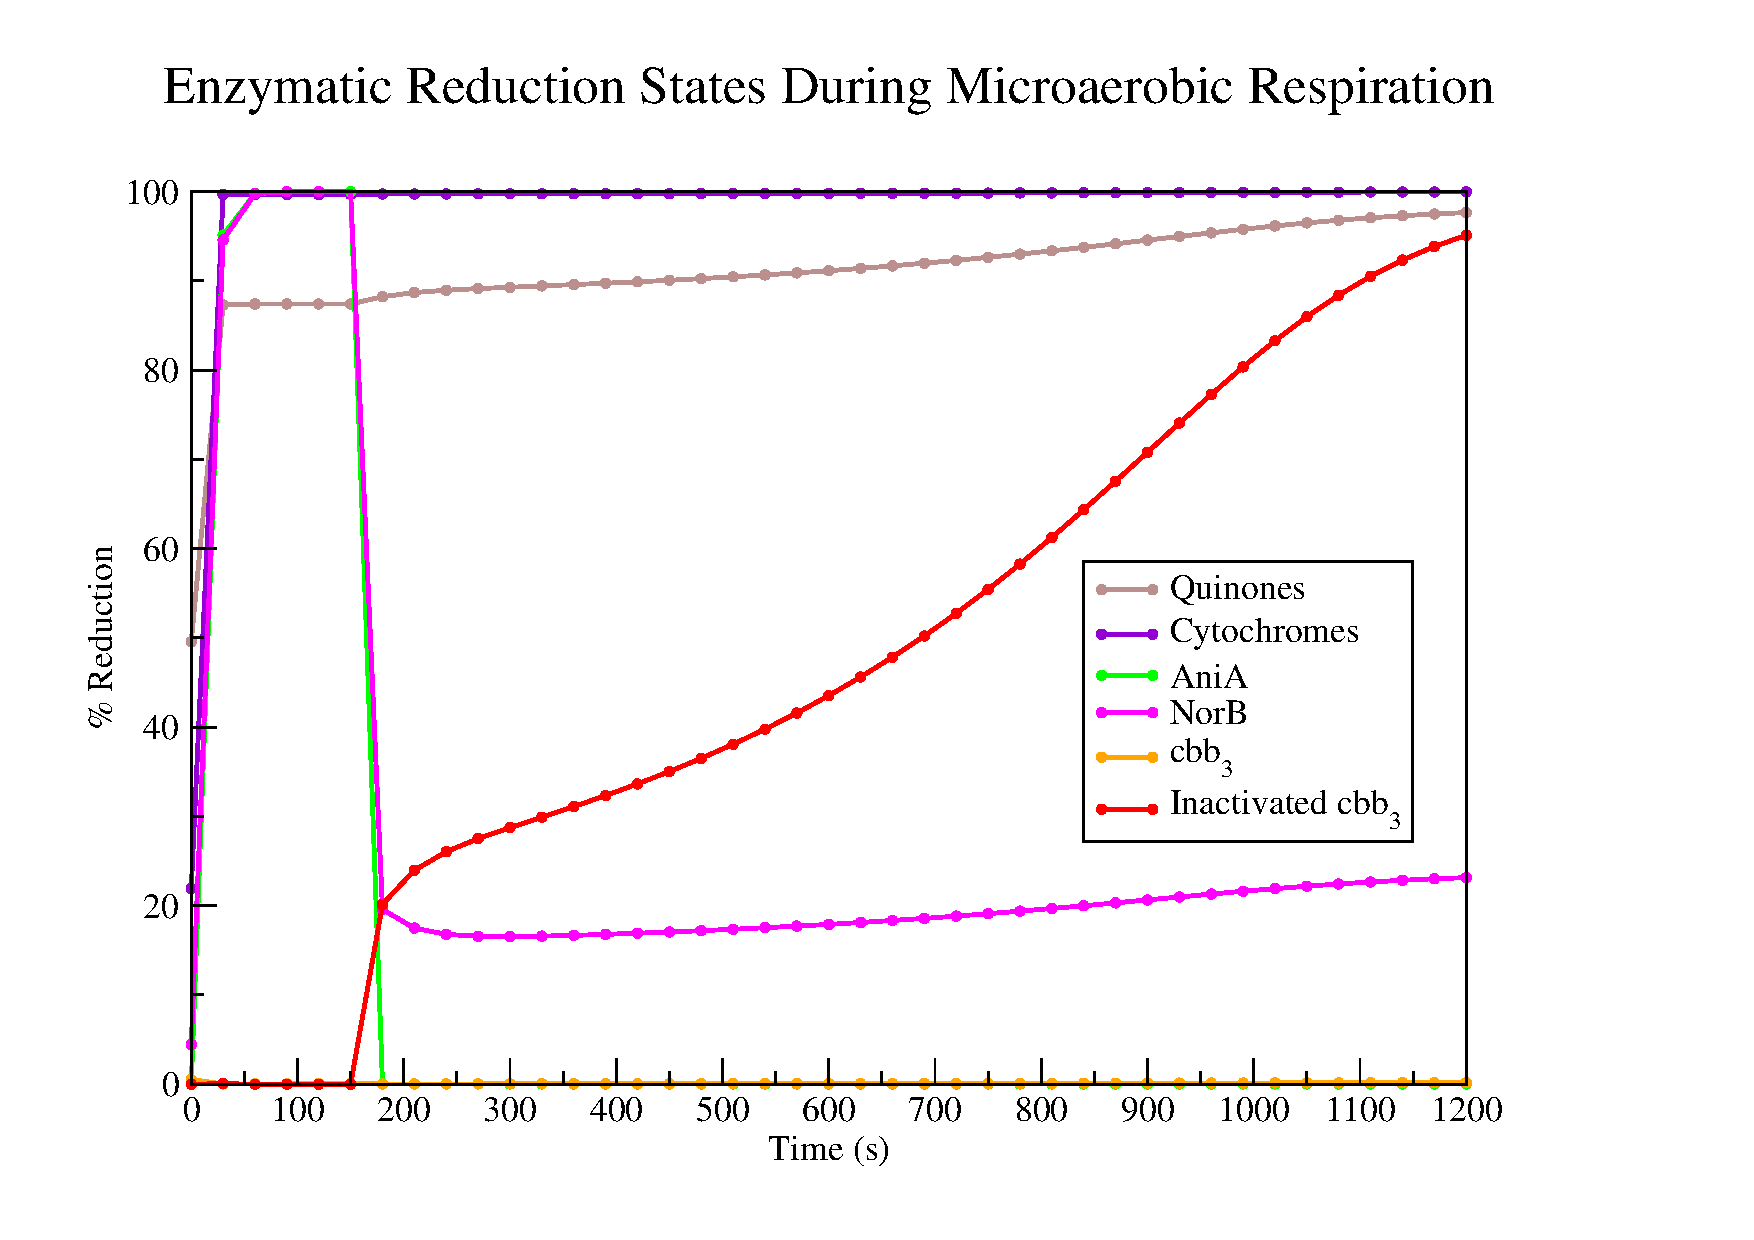
\includegraphics[height=10cm, trim=1cm 1cm 3cm 1cm, clip=true]{./07-nitritereduction/data/dataset2redox-1.pdf}
 % dataset2redox-1.pdf: 842x595 pixel, 72dpi, 29.70x20.99 cm, bb=0 0 842 595
 \caption[Reduction States During Nitrite Reduction]{{\bf Reduction States During Nitrite Reduction}. This figure shows how the reduction states of the enzymes involved in nitrite reduction change during respiration.
  \label{fig:nitrite_ds2_redox1}}
\end{figure}

\subsection{Discussion}

Re-run simulations: my data broaden k1 and k3 and same for l1 l3 to try and fix both o2 reduction rate an no-non-reduction. C maybe needs to decrease. NO reduction rate should roughly equal O2 reduction rate (in denitrifying conditions) according to \citet{Rock2005}. Therefore l1*B should equal k1*C ish.
Rock data reset to zero and reduce f and g to try and get Q and X to be less reduced to trigger an increase in NO when O2 runs out. Q pool redox states differ (in paracoccus) \cite{Otten1999}.

Plot again with redox states to confirm or reject.

These changes will no doubt break the previous results (o2 and NO), but that is not necessarily a huge problem. The model seems capable of simulating the effect of nitric oxide on oxygen reduction rate, but in order to effect the changes in microaerobic conditions more drastic changes have to be made. This is quite likely as a result of the simplification of the redox chain in that all cytochromes are treated as one entity rather than the 4ish that actually exist. With all cytochromes modelled individually the potential redox state of bc1 could be different to that of cx,c4,c5 which could negate the need to alter f and g to lower the overall reduction state of X. If this is the case it goes a way to explain why the redox chain appears to be so complicated \textit{in vivo} rather than just have 1 serve-all cytochrome. Sadly this is something that was not possible to investigate in this study but could be included in further work onthe subject.
